% Based on Models 1 and 2 in "Searching" by Clif Kussmaul

\model{Hi-Lo Game}

\begin{wrapfigure}{r}{0.4\textwidth}
\centering
\vspace{-1em}
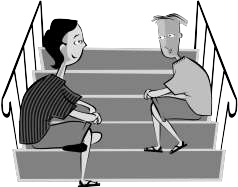
\includegraphics[width=\linewidth]{CSP/hi-low1.png}
\vspace*{-4em}
\end{wrapfigure}

Hi-Lo is a number guessing game with simple rules, played by school children.
\vspace{1ex}
\begin{enumerate}[nosep]
\item There are two players -- $A$ and $B$.
\item Player $A$ thinks of a number from 1 to 100.
\item Player $B$ guesses a number.
\item Player $A$ responds with \\ ``too high'', ``too low'', or ``you win''.
\item Players $B$ and $A$ continue to guess and \\ respond until $B$ wins (or gives up).
\end{enumerate}


\quest{12 min}


\Q How many different answers can player $A$ give?

\vspace{1ex}


\Q When does the game end?

\begin{answer}[2em]
\end{answer}


\Q Play the game a few times to ensure that everyone understands the rules.

\vspace{1ex}

\begin{center}
\begin{tabularx}{\linewidth}{|X|}
\hline
\it
In computing, we often must search in a set for a particular item.
As computer scientists, we are particularly interested in searching very large sets, with thousands or millions of values.
For example, the Harvard University Library has roughly 16,000,000 volumes, and the US Library of Congress has roughly 22 million cataloged books and over 100,000,000 total items.
\\
\hline
\end{tabularx}
\end{center}


\Q Identify 4--5 different guessing strategies that Player $B$ could use.
Each strategy should describe a \textbf{different approach} to the game.
For example: \textit{Start at 1, and count up until the correct answer is found.}
Try to have a mixture of simple and clever approaches, including ones that young children could use.

\begin{enumerate}
\item 
\item 
\item 
\item 
\item 
\end{enumerate}


\Q Rank order the algorithms with regard to how \textbf{fast} it will find the right answer.
Write 1 for the fastest strategy (fewest guesses) and 5 for the slowest one (most guesses).

\begin{answer}
\end{answer}


\Q Rank order each strategy with regard to how \textbf{easy} it is to describe or specify.
(Suppose you had to explain each approach to a first-grader so that she could play the game.)
Write 1 for the strategy that is easiest to describe, and 5 for the one that is hardest.

\begin{answer}
\end{answer}


\Q For each strategy ($a$ to $e$), plot its fast and easy values on the graph below:

\begin{table}[h]
\centering
\renewcommand{\arraystretch}{1.6}
\begin{tabularx}{275pt}{X C{28pt} | C{28pt} C{28pt} C{28pt} C{28pt} C{28pt}}
Hard & 5 \\
     & 4 \\
     & 3 \\
     & 2 \\
Easy & 1 \\
\hline
     & & 1    & 2 & 3 & 4 & 5    \\
     & & Fast &   &   &   & Slow \\
\end{tabularx}
\end{table}


\Q In complete sentences, describe the relationship between the fast and easy rankings, including what you see from the graph. 

\begin{answer}
\end{answer}
